\label{chap:introduction}

\section{Contextualização}

Os Fundos de Investimento Imobiliário, comumente conhecidos como FII, são formados por um grupo de pessoas/investidores, que tem por objetivo, destinar seus recursos financeiros em ativos imobiliários, seja para o desenvolvimento de empreendimentos ou em imóveis prontos que podem ser prédios ou edifícios comerciais, como shoppings, hospitais, faculdades etc. A intenção dos FIIs é de obter retorno de rendimentos através da locação, arrendamento ou venda destes imóveis ou de rendimento de outros títulos financeiros imobiliários. O montante de recursos destinados ao fundo são particionados e distribuídos aos investidores em forma de cotas. O investidor pode negociar suas cotas, comprando ou vendendo através da bolsa de valores.
Existem dois tipos de fundos imobiliários:

\begin{itemize}
  \item Fundos de tijolo
    \begin{itemize}
      \item Focados em empreendimentos físicos. Suas estratégias administrativas são voltadas para a aquisição, construção e aluguéis de imóveis comerciais. O objetivo desta categoria de fundo é de encontrar potenciais locatários a fim de rentabilizar o fundo através dos aluguéis. 
    \end{itemize}
  \item Fundos de papéis
  \begin{itemize}
    \item Focados no reinvestimento dos recursos do fundo em títulos financeiros vinculados ao mercado imobiliário como LCI (Letra de Crédito Imobiliário), CRI (Certificados de Recebíveis Imobiliários), títulos recebíveis e cotas de outros Fundos Imobiliários. Os rendimentos destes títulos financeiros refletem ao rendimento do Fundo administrado.
  \end{itemize}
\end{itemize}

Cada FII tem sua administradora que faz a gestão das cotas do fundo. Por via de regra, os administradores devem destinar 95\% dos rendimentos do Fundo aos investidores detentores das cotas.

A lucratividade de um FII é oriunda da valorização de suas cotas através das negociações na bolsa de valores  e/ou na distribuição dos rendimentos adquiridos ao longo do tempo em forma de dividendos.
De acordo com os dados divulgados pelo ANBIMA, o número de emissões de FIIs no primeiro trimestre de 2019, alcançou a marca de R\$ 6,4 bilhões contra R\$ 3,2 bilhões no mesmo período em 2018, o que representou um crescimento no volume de mais de 97\%. 

Diante dessas informações percebe-se a melhora do segmento imobiliário e aumento na procura dos fundos viabilizada pela diminuição dos níveis das taxas de juros. A figura~\ref{fig:real_estate_investment}, demonstra o panorama mencionado. Esse crescimento acelerado deve-se também em parte a baixa taxa de juros de mercado e a um cenário de retração econômica nacional. 

\begin{center}
\begin{figure}
\begin{centering}
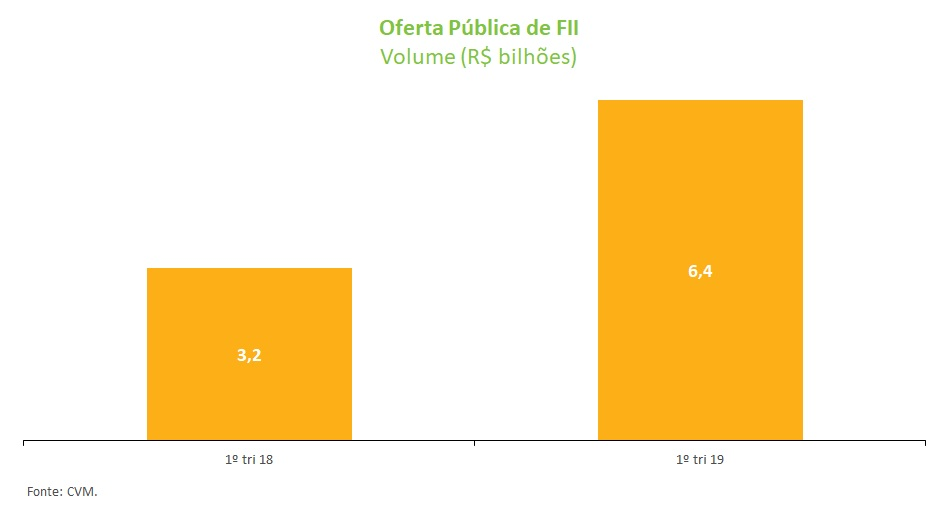
\includegraphics[width=1.0\textwidth]{InvestimentoDoMercadoImobiliario}
\end{centering}
\caption{\label{fig:real_estate_investment}Demonstração do investimento total bruto do mercado imobiliário no Brasil no T1/2018 em relação ao T1/2019.}
\end{figure}
\vspace*{-44pt}
\end{center}

\begin{center}
\begin{figure}
\begin{centering}
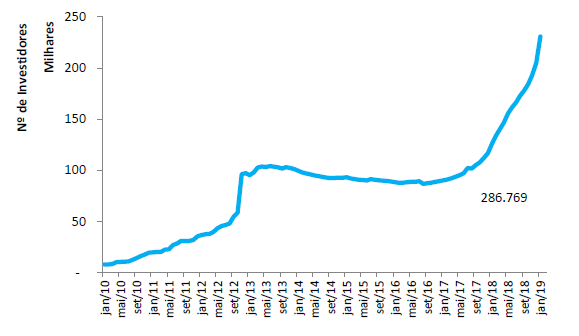
\includegraphics[width=1.0\textwidth]{InvestidoresDoMercadoImobiliario}
\end{centering}
\caption{\label{fig:real_estate_investors}Número de investidores do mercado imobiliário no Brasil entre Janeiro/2010 e Janeiro/2019.}
\end{figure}
\vspace*{-44pt}
\end{center}

Em análise do boletim de Mercado Imobiliário de março/2019 divulgado pela B3, da figura~\ref{fig:real_estate_investors}, observa-se um relevante aumento de investidores entre Janeiro de 2018 à Janeiro de 2019, alcançando o número de 286.796 pessoas. 

Em meio ao crescimento do número de fundos negociados em mercado e o grande aumento da procura por parte dos investidores destes produtos, é importante, ter embasamento de estudos a fim de destacar quais fundos são mais rentáveis e quais valem a pena o esforço de recursos financeiros oferecidos pelos investidores aos gestores e administradores. 
A base de análise deste presente estudo evidenciará os fundos de tijolos na intenção de auxiliar o investidor na obtenção de informações através da relação dos fundos mais rentáveis com a localização dos seus ativos.
Fundos com ativos localizados em regiões com mais desenvolvimento tendem a ter menor vacância e seus aluguéis mais valorizados.

\section{Objetivo Geral}

Prover um mecanismo para que investidores de fundos imobiliários de tijolos a escolherem produtos que possuam ativos em determinadas localizações que tendem a se valorizar, comparando-os com outros fundos que também possuam empreendimentos nos mesmos locais e que historicamente tenham bons rendimentos. 
O estudo avaliará, pela geolocalização, rendimentos e pela valorização das cotas se determinados fundos possuem correlação com a região em que estão alocados ou com fundos semelhantes na mesma região.
